%! Author = bedlamzd
%! Date = 28.02.2021

% Preamble
\documentclass[14pt]{extarticle}

%! Author = bedlamzd
%! Date = 16.02.2021

\usepackage{fontspec}
\usepackage{polyglossia}
\defaultfontfeatures{Ligatures=TeX}
\setdefaultlanguage{russian}
\setotherlanguage{english}
\setmainfont{PT Astra Serif}
\newfontfamily{\latinfont}{PT Astra Serif}
\newfontfamily{\cyrillicfont}{PT Astra Serif}
\newfontfamily{\cyrillicfonttt}{FreeMono}

\usepackage{geometry}

\usepackage{amsmath}
\usepackage{amssymb}
\usepackage{amsfonts}
\usepackage{graphicx}
\usepackage{float}
\usepackage{wrapfig}
\usepackage[caption=false]{subfig}

\geometry{right=20mm}
\geometry{left=20mm}
\geometry{top=20mm}
\geometry{bottom=20mm}

\usepackage{indentfirst}
\usepackage[outputdir=out]{minted}

\renewcommand{\theFancyVerbLine}{\ttfamily{\normalsize\oldstylenums{\arabic{FancyVerbLine}}}}

\newminted{python}{autogobble, linenos, fontsize=\small, xleftmargin=2\parindent}
\newmintinline{python}{fontsize=\small}
\newmintedfile{python}{autogobble, linenos, fontsize=\small, xleftmargin=2\parindent,
breakanywhere, breaklines}

\newminted{matlab}{autogobble, linenos, fontsize=\small, xleftmargin=2\parindent}
\newmintinline{matlab}{fontsize=\small}
\newmintedfile{matlab}{autogobble, linenos, fontsize=\small, xleftmargin=2\parindent,
breakanywhere, breaklines}

\renewcommand{\thesubsection}{\arabic{subsection}}

\graphicspath{{../img/}}



% Document
\begin{document}
    \begin{titlepage}
    \begin{center}
        \begin{small}
            \textbf{Министерство науки и высшего образования Российской Федерации}

            \vspace{1em}

            ФЕДЕРАЛЬНОЕ ГОСУДАРСТВЕННОЕ АВТОНОМНОЕ ОБРАЗОВАТЕЛЬНОЕ\\
            УЧРЕЖДЕНИЕ ВЫСШЕГО ОБРАЗОВАНИЯ

            \vspace{1em}

            \textbf{<<НАЦИОНАЛЬНЫЙ ИССЛЕДОВАТЕЛЬСКИЙ УНИВЕРСИТЕТ ИТМО>>}
        \end{small}

        \vspace{13ex}

        Практическая работа №4\\
        <<Планирование движения>>\\
        по дисциплине <<Моделирование и управление робототехническими системами>>
    \end{center}

    \vspace{14em}

    \begin{flushright}
        \noindent
        Выполнил:\\
        студент гр. R41341c\\
        Борисов М. В.

        \vspace{1em}
        Преподаватель:\\
        Каканов М. А.
    \end{flushright}

    \vfill

    \begin{center}
        \large{Санкт-Петербург}\\
        2021 г.\\
    \end{center}
\end{titlepage}


    \section*{Дано}

    \section*{Задание}
    Построить матрицу Якоби и решить ПЗК и ОЗК по скорости для шестизвенного манипулятора.

    \section*{Решение}
    Системы координат выбраны как показано на рисунке~\ref{pic:frames}
    \begin{figure}[H]
        \centering
        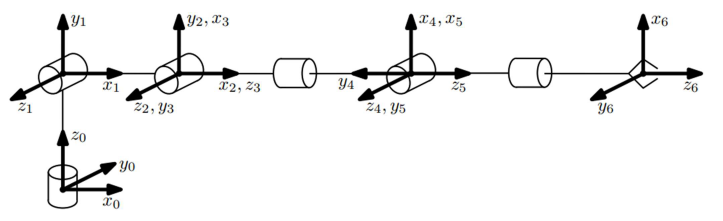
\includegraphics[width=0.75\textwidth]{frames.png}
        \caption{Системы координат звеньев манипулятора}
        \label{pic:frames}
    \end{figure}

    Параметры Денавита-Хартенберга приведены в таблице~\ref{tbl:params}.
    Значения параметров $a_i,\ d_i$ были приняты единычными. Поскольку все звенья манипулятора
    вращательные, то углы $\theta_i$ выступают в качестве обобщённых координат и будут выбраны произвольно.
    {
    \renewcommand{\arraystretch}{2}
    \begin{table}[H]
        \centering
        \begin{tabular}{*{5}{c}}\toprule
            Звено, $i$  & $a_i$ & $\alpha_i$        & $d_i$ & $\theta_i$ \\ [1ex] \midrule
            1           & 0     & $\dfrac{\pi}{2}$  & $d_1$ & $\theta_1$ \\ [1ex] \midrule
            2           & $a_2$ & 0                 & 0     & $\theta_2$ \\ [1ex] \midrule
            3           & 0     & $\dfrac{\pi}{2}$  & 0     & $\theta_3 + \dfrac{\pi}{2}$ \\ [1ex] \midrule
            4           & 0     & $-\dfrac{\pi}{2}$ & $d_4$ & $\theta_4$ \\ [1ex] \midrule
            5           & 0     & $\dfrac{\pi}{2}$  & 0     & $\theta_5$ \\ [1ex] \midrule
            6           & 0     & 0                 & $d_6$ & $\theta_6$ \\ [1ex]
            \bottomrule
        \end{tabular}
        \caption{Параметры Денавита-Хартенберга}
        \label{tbl:params}
    \end{table}
    }

    В приложении~\ref{code:jacob} приведена функция для решения обратной задачи кинематики. В нём задаются параметры
    манипулятора и производится расчёт.

    После инициализации значений манипулятора строятся матрицы трансформации $T$ для каждого звена манипулятора в символьном виде.

    Затем строится матрица Якоби, в которой каждой столбец вычисляется как частная производная из линейной и угловой компоненты вектора.
    Линейная компонента есть частная производная вектора координат $p^0_n$ по $q_i$, где вектор координат находится из ранее
    рассчитанных матриц $T$. Угловая компонента есть три строчки третьего столбца тех же матриц $T$.

    Матрица Якоби таким образом выглядит
    \begin{equation}
        J =
        \begin{bmatrix}
            J_{v_1}(1) \dots J_{v_6}(q) \\
            J_{\omega_1}(1) \dots J_{\omega_6}(q)
        \end{bmatrix}
    \end{equation}

    В итоге в данную матрицу (которая найденна в символьном виде) подставляются реальные значения и получается
    конкретный ответ.

    Решим теперь ПЗК и ОЗК.
    \begin{matlabcode*}{frame=single, xleftmargin=\parindent}
        >> J = jacob([0.28 0.2 0.1 0.9 0.9 0.9])

        J =

            0.0579    1.1596    1.3506   -0.4288    0.2669         0
            2.0191    0.3335    0.3884   -0.6300   -0.4299         0
                 0    1.9245    0.9444   -0.1813    0.8625         0
                 0    0.2764    0.2764    0.2840   -0.5474    0.7932
                 0   -0.9611   -0.9611    0.0817   -0.8042   -0.4104
            1.0000    0.0000    0.0000   -0.9553   -0.2315   -0.4500

        >> J * [0.28 0.2 0.1 0.9 0.9 0.9]'

        ans =

            0.2374
           -0.2830
            1.0924
            0.5597
           -1.3079
           -1.1931

        >> inv(J)*ans

        ans =

            0.2800
            0.2000
            0.1000
            0.9000
            0.9000
            0.9000
    \end{matlabcode*}

    Решение ОЗК соответствует входным аргументам ПЗК, что доказывает правильность реализации.

    \section*{Вывод}
    В ходе работы написана функция вычисляющая фиксированную матрицу Якоби для шестизвенного манипулятора и позволяющая
    с её помощью решать прямую и обратную задачу кинематики по скорости.

    \appendix \newpage
    \renewcommand{\thesection}{\Asbuk{section}}
    \section{Функция решения прямой задачи кинематики}\label{code:jacob}
    \octavefile[frame=single]{../src/jacob.m}

\end{document}
